\documentclass[dvipdfmx,12pt]{beamer}
\usetheme{Copenhagen}
\usefonttheme{professionalfonts}

\usepackage{bxdpx-beamer}
\usepackage{pxjahyper}
\renewcommand\kanjifamilydefault{\gtdefault}
\renewcommand\familydefault{\sfdefault}

\setbeamertemplate{navigation symbols}{}
% \setbeamertemplate{footline}[frame number]
\setbeamercolor{page number in head/foot}{fg=gray}
\setbeamerfont{page number in head/foot}{size=\small}
\setbeamerfont{title}{size=\Large}
\setbeamerfont{author}{size=\large}
\setbeamerfont{institute}{size=\normalsize}
\setbeamerfont{date}{size=\normalsize}
\setbeamertemplate{footnote}{
  \parindent 0em\noindent
  \raggedright
  \usebeamercolor{footnote}\hbox to 0.8em{\hfil\insertfootnotemark}\insertfootnotetext\par%
}

\usepackage{amsmath}
\usepackage{amssymb}
\usepackage{makecell}
\usepackage{url}

\title{Distortion Camera}
\author{
  {\small 数理・計算科学系} 金子孟司
}
\institute{ソフトウェア開発演習 個人プロジェクト制作物デモ大会}
\date{Jul. 1, 2019}
\titlegraphic{
  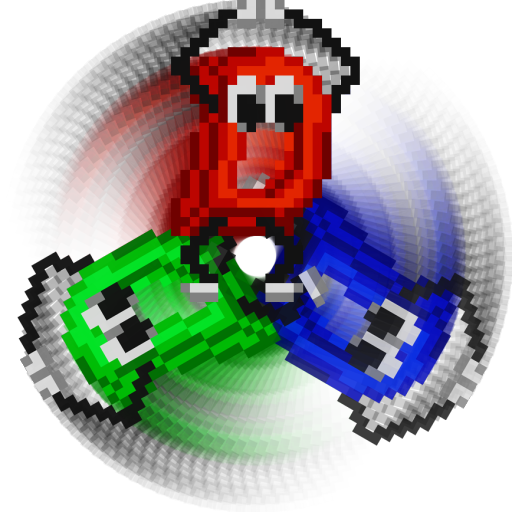
\includegraphics[width=0.15\linewidth]{fig/ark.png}
}

\begin{document}

\setbeamertemplate{footline}{}
\frame[noframenumbering]{\maketitle}
\setbeamertemplate{footline}[frame number]


\begin{frame}{概要}
  \begin{columns}[c]
    \begin{column}{0.6\linewidth}
      \begin{block}{これはなに}
        センサに反応して空間を歪ませながら撮影できるカメラ
      \end{block}
      \begin{itemize}
        \item 開発言語:Kotlin,GLSL
        \item 制作期間:2日間
        \item URL:\url{https://github.com/ArkArk/DistortionCamera}
      \end{itemize}
      \begin{exampleblock}{どんな人向けのアプリか}
        \begin{itemize}
          \item 普通のカメラに飽きた人
          \item シェーダでエンジョイしたい人
          \item 線形な世界に消耗している人
        \end{itemize}
      \end{exampleblock}
    \end{column}
    \begin{column}{0.4\linewidth}
      \begin{center}
        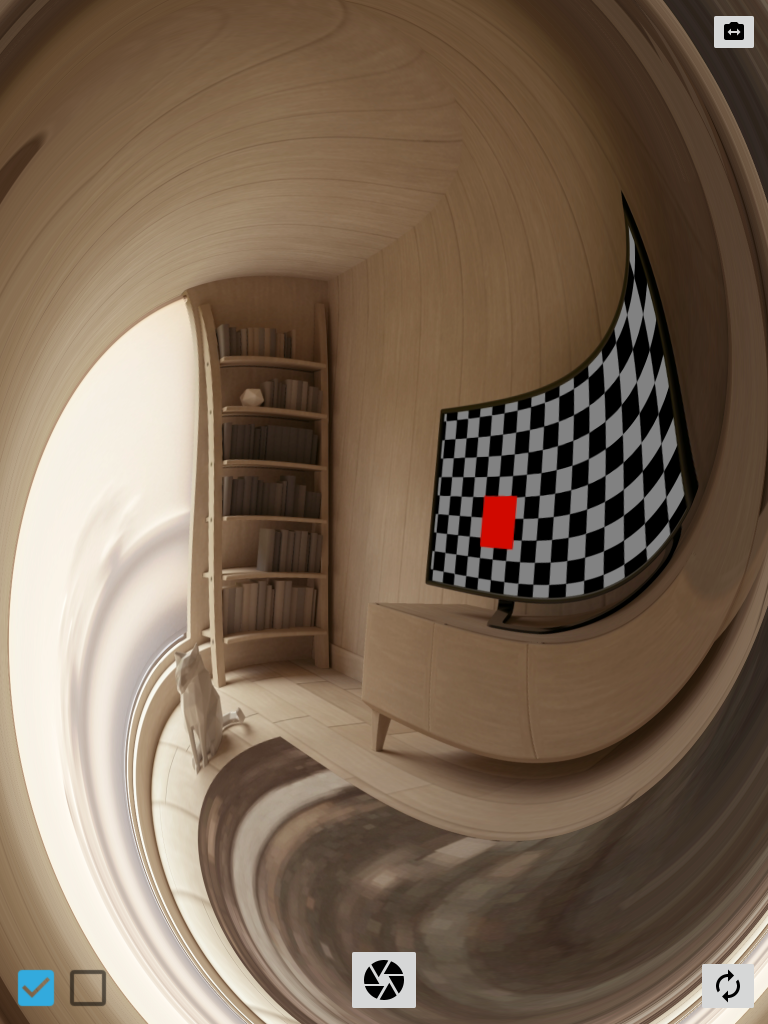
\includegraphics[width=\linewidth]{fig/screenshot.png}
      \end{center}
    \end{column}
  \end{columns}
\end{frame}


\begin{frame}{構成}
  \begin{center}
    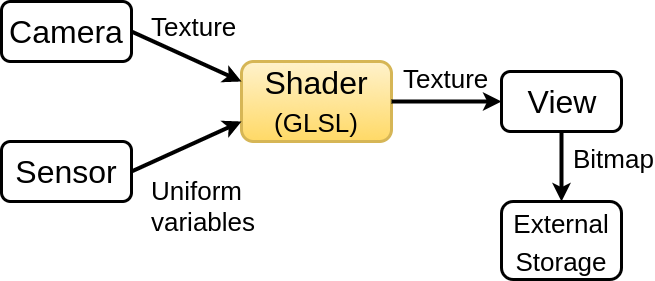
\includegraphics[width=0.75\linewidth]{fig/structure.png}
  \end{center}
  \begin{block}{}
    \begin{enumerate}
      \item 各情報をShader側へ流す
      \begin{itemize}
        \item テクスチャ:カメラのプレビュー
        \item ユニフォーム変数:センサーに関する値
      \end{itemize}
      \item シェーダの結果を画面に表示
      \item ビットマップに変換してストレージに保存
    \end{enumerate}
  \end{block}
\end{frame}


\begin{frame}{Shader}
  Shader(fragment shader)内でやっていることの例
  \begin{columns}[c]
    \begin{column}{0.7\linewidth}
      \begin{enumerate}
        \item 座標を$\textit{uv} \in [-1, 1] \times [-1, 1]$に正規化
        \item 回転行列をかけて座標変換:$\textit{uv} \leftarrow \textit{rotate}(\textit{uv}, t)$
        \begin{itemize}
          \item 角度$t$は次の値に依存:
          \begin{itemize}
            \item $\textit{len}(\textit{uv})$
            \item センサの値
          \end{itemize}
        \end{itemize}
        \item テクスチャの色をとってくる
        \begin{itemize}
          \item $\textit{texture2D}(\textit{camTexture}, \textit{uv} \cdot 0.5 + 0.5)$
        \end{itemize}
      \end{enumerate}
    \end{column}
    \begin{column}{0.3\linewidth}
      \begin{center}
        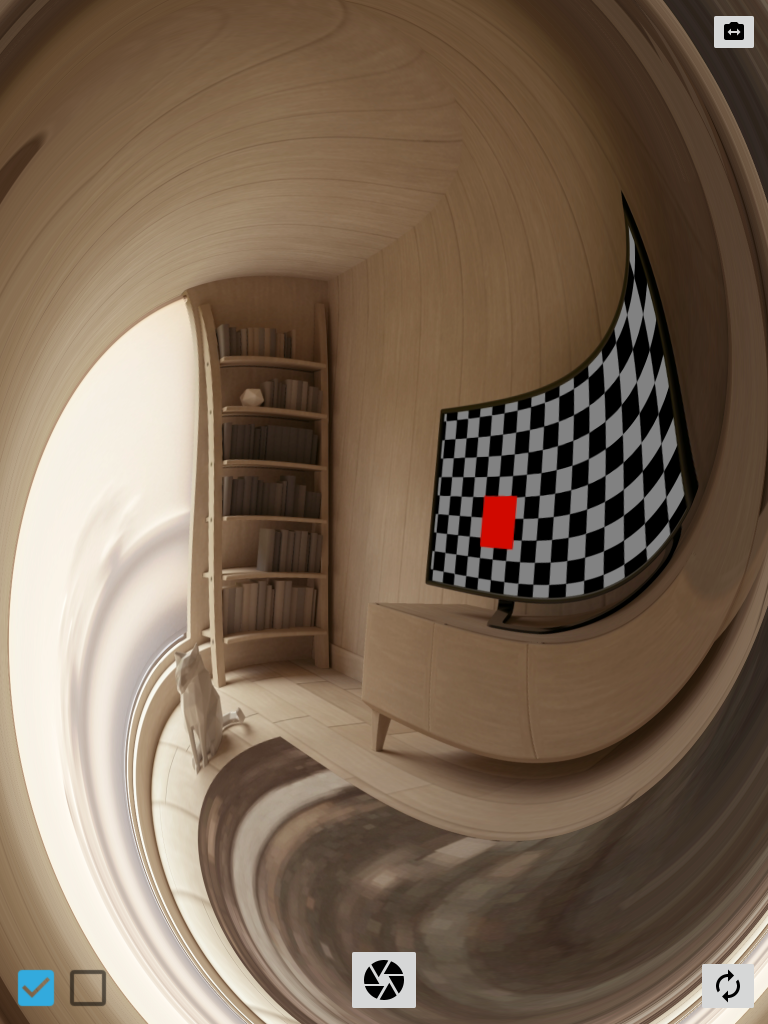
\includegraphics[width=\linewidth]{fig/screenshot.png}
      \end{center}
    \end{column}
  \end{columns}
\end{frame}


\definecolor{lightblue}{rgb}{0.88, 0.91, 1.0}
{\setbeamercolor{background canvas}{bg=lightblue}
  \begin{frame}[c]
    \begin{center}
      \Large デモ
    \end{center}
  \end{frame}
}


\begin{frame}{まとめ}
  \begin{columns}[c]
    \begin{column}{0.7\linewidth}
      センサに反応して歪むカメラを実装した
      \begin{itemize}
        \item フラグメントシェーダをいじるだけで自由度の高い表現が可能
        \item $\rightarrow$ たとえば万華鏡カメラもつくれる
      \end{itemize}
    \end{column}
    \begin{column}{0.3\linewidth}
      \begin{center}
        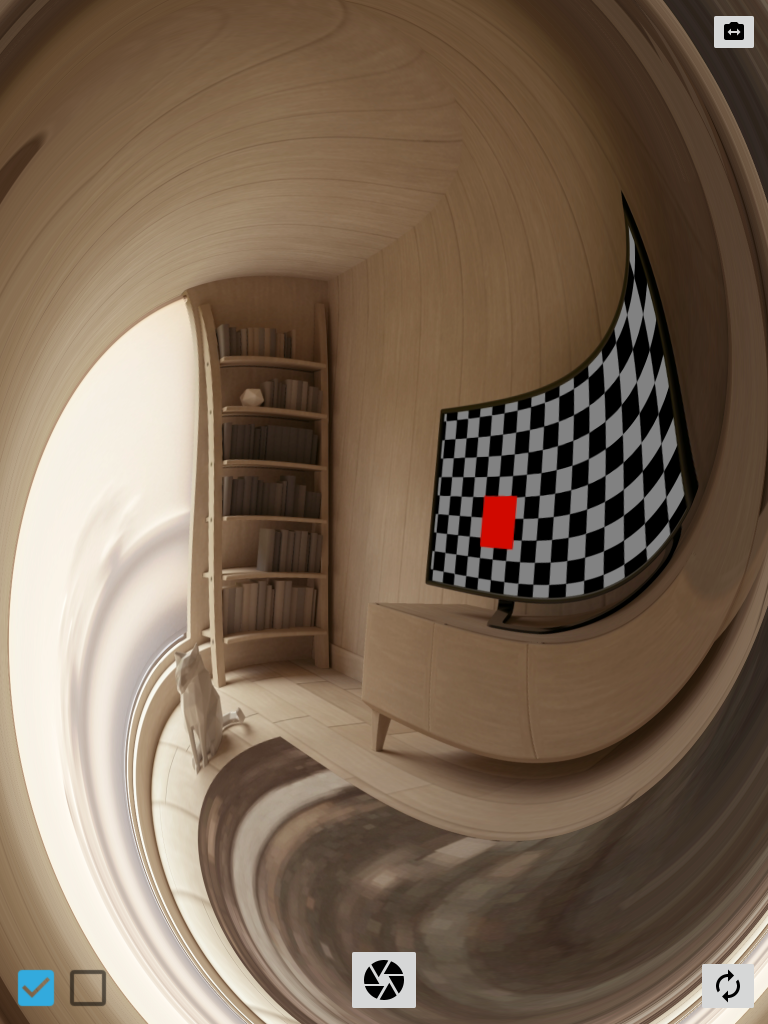
\includegraphics[width=\linewidth]{fig/screenshot.png}
      \end{center}
    \end{column}
  \end{columns}
\end{frame}


\end{document}
